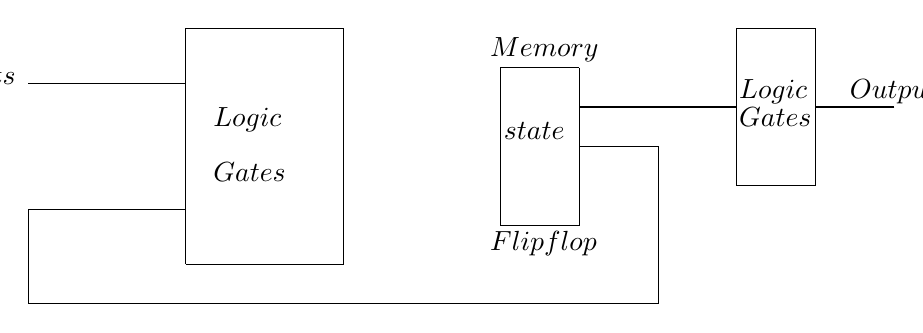
\begin{tikzpicture}


\draw (0,0.7)--(-2,0.7);
\draw (0,2.3)--(-2,2.3);
\draw (0,0) -- (2,0) -- (2,3) -- (0,3) -- (0,0);
\draw (5,1.5)--(6,1.5);
\draw (5,2.5)--(5,0.5)--(4,0.5)--(4,2.5)--(5,2.5);
\draw (6,1.5)--(6,-0.5);
\draw (6,-0.5)--(-2,-0.5);
\draw (-2,0.7)--(-2,-0.5);
\draw (5,2)--(7,2);
\draw (7,3)--(7,1);
\draw (7,3)--(8,3)--(8,1)--(7,1);
\draw (9,2)--(8,2);

\put (110,75) {$Memory$}
\put (115,45) {$state$}
\put (-90,65) {$inputs$}
\put (10,50) {$Logic$}
\put (10,30) {$Gates$}
\put (200,60) {$Logic$}
\put (200,50) {$Gates$}
\put (240,60) {$Output$};
\put (110,5) {$Flip flop$}

\end{tikzpicture}